\documentclass[aspectratio=169,10pt]{beamer}

% Theme and typography
\usetheme{default}
\usecolortheme{default}
\setbeamertemplate{navigation symbols}{}

% Color definitions
\usepackage{xcolor}
\definecolor{Navy}{HTML}{0F2042}
\definecolor{NavyLight}{HTML}{1E3A8A}
\definecolor{CyanAccent}{HTML}{0284C7}
\definecolor{CyanLight}{HTML}{E0F2FE}
\definecolor{SlateDark}{HTML}{1E293B}
\definecolor{SlateMuted}{HTML}{64748B}
\definecolor{LightBg}{HTML}{F8FAFC}
\definecolor{BorderCol}{HTML}{CBD5E1}
\definecolor{AlertRed}{HTML}{DC2626}
\definecolor{SuccessGreen}{HTML}{059669}

\setbeamercolor{frametitle}{fg=Navy,bg=white}
\setbeamercolor{title}{fg=Navy}
\setbeamercolor{structure}{fg=NavyLight}
\setbeamercolor{normal text}{fg=SlateDark}
\setbeamercolor{item}{fg=CyanAccent}
\setbeamercolor{subitem}{fg=NavyLight}

% Footnote reference mechanism
\newcommand{\slideref}[1]{\gdef\currentref{#1}}
\gdef\currentref{}

\setbeamertemplate{footline}{%
  \leavevmode%
  \begin{beamercolorbox}[wd=\paperwidth,leftskip=0.8cm,rightskip=0.8cm]{normal text}%
    \ifx\currentref\empty\else%
      {\fontsize{6}{7.2}\selectfont\color{SlateMuted}\textbf{Ref:} \currentref\par\vskip1.5pt}%
    \fi%
    {\fontsize{7}{8}\selectfont\color{SlateMuted}Carnegie Mellon Forum on Biomedical Engineering 2026 \enspace$\cdot$\enspace Abstract \#194%
    \hfill%
    \bfseries\color{NavyLight}Slide \insertframenumber{} of \inserttotalframenumber}%
  \end{beamercolorbox}%
  \vskip3pt%
  \gdef\currentref{}%
}

\usepackage{graphicx}
\usepackage{booktabs}
\usepackage{tcolorbox}
\tcbuselibrary{skins}

\tcbset{
  cardstyle/.style={
    enhanced, colback=LightBg, colframe=BorderCol, boxrule=1pt, arc=2mm,
    left=3mm, right=3mm, top=2mm, bottom=2mm, coltitle=white
  }
}

% Title metadata
\title{\textbf{\LARGE Can We Reconstruct a Diagnostic 12-Lead ECG from Only a Few Measured Leads?}}
\subtitle{\vspace{0.2em}\color{SlateMuted}\normalsize Discrete Latent Sequence Generation for 12-Lead ECG Reconstruction from Limited Leads}
\author{\textbf{Mithun Manivannan, BSc}$^{1,2}$ \and \textbf{Alex Mariakakis, PhD}$^{1}$ \and \textbf{Christopher Cheung, MD}$^{2}$}
\institute{$^{1}$Department of Computer Science, University of Toronto \quad $^{2}$Division of Cardiology, Sunnybrook Health Sciences Centre}
\date{\footnotesize\color{CyanAccent}\textbf{2026 Carnegie Mellon Forum on Biomedical Engineering \enspace$\cdot$\enspace Abstract \#194}}

\begin{document}

% =========================================================================
% Slide 1: Question
% =========================================================================
\begin{frame}[plain]
  \vspace{0.6em}
  \begin{columns}[c]
    \begin{column}{0.48\textwidth}
      
\includegraphics[height=0.95cm,keepaspectratio]{figures/logos/uoft_cs_logo.png}
    \end{column}
    \begin{column}{0.48\textwidth}
      \hfill
\includegraphics[height=0.95cm,keepaspectratio]{figures/logos/sunnybrook_logo.png}
    \end{column}
  \end{columns}

  \vskip 1.0em
  \centering
  {\fontsize{19}{24}\selectfont\textbf{\color{Navy}Can We Reconstruct a Diagnostic 12-Lead ECG\\from Only a Few Measured Leads?}\par}
  \vskip 0.6em
  {\fontsize{11}{14}\selectfont\color{SlateMuted}Discrete Latent Sequence Generation for Limited-Lead ECG Reconstruction\par}

  \vskip 1.2em
  \begin{tcolorbox}[cardstyle,colframe=BorderCol,top=3.5mm,bottom=3.5mm]
    \centering
    {\fontsize{10.5}{13.5}\selectfont\textbf{Mithun Manivannan, BSc}$^{1,2}$ \quad \textbf{Alex Mariakakis, PhD}$^{1}$ \quad \textbf{Christopher Cheung, MD}$^{2}$\par}
    \vskip 0.3em
    {\fontsize{8.5}{11}\selectfont\color{SlateMuted}$^{1}$Department of Computer Science, University of Toronto \quad $^{2}$Division of Cardiology, Sunnybrook Health Sciences Centre\par}
    \vskip 0.4em
    {\fontsize{8.5}{11}\selectfont\bfseries\color{CyanAccent}2026 Carnegie Mellon Forum on Biomedical Engineering \enspace$\cdot$\enspace Abstract \#194\par}
  \end{tcolorbox}
  \note{Hello everyone. I’m Mithun Manivannan from the University of Toronto and Sunnybrook Health Sciences Centre. Today I am presenting our work asking a fundamental question: can we reconstruct a full diagnostic twelve-lead electrocardiogram from only a few measured wearable leads?}
\end{frame}

% =========================================================================
% =========================================================================
% Slide 2: 12 Leads vs. One Wearable Lead
% =========================================================================
\begin{frame}{12 Leads vs. One Wearable Lead}
  \slideref{Perez et al., Apple Heart Study, \textit{N Engl J Med} 2019; Cheung et al., \textit{Heart Rhythm} 2023.}
  \vspace{-0.3em}
  \begin{columns}[T]
    \begin{column}{0.53\textwidth}
      \centering
      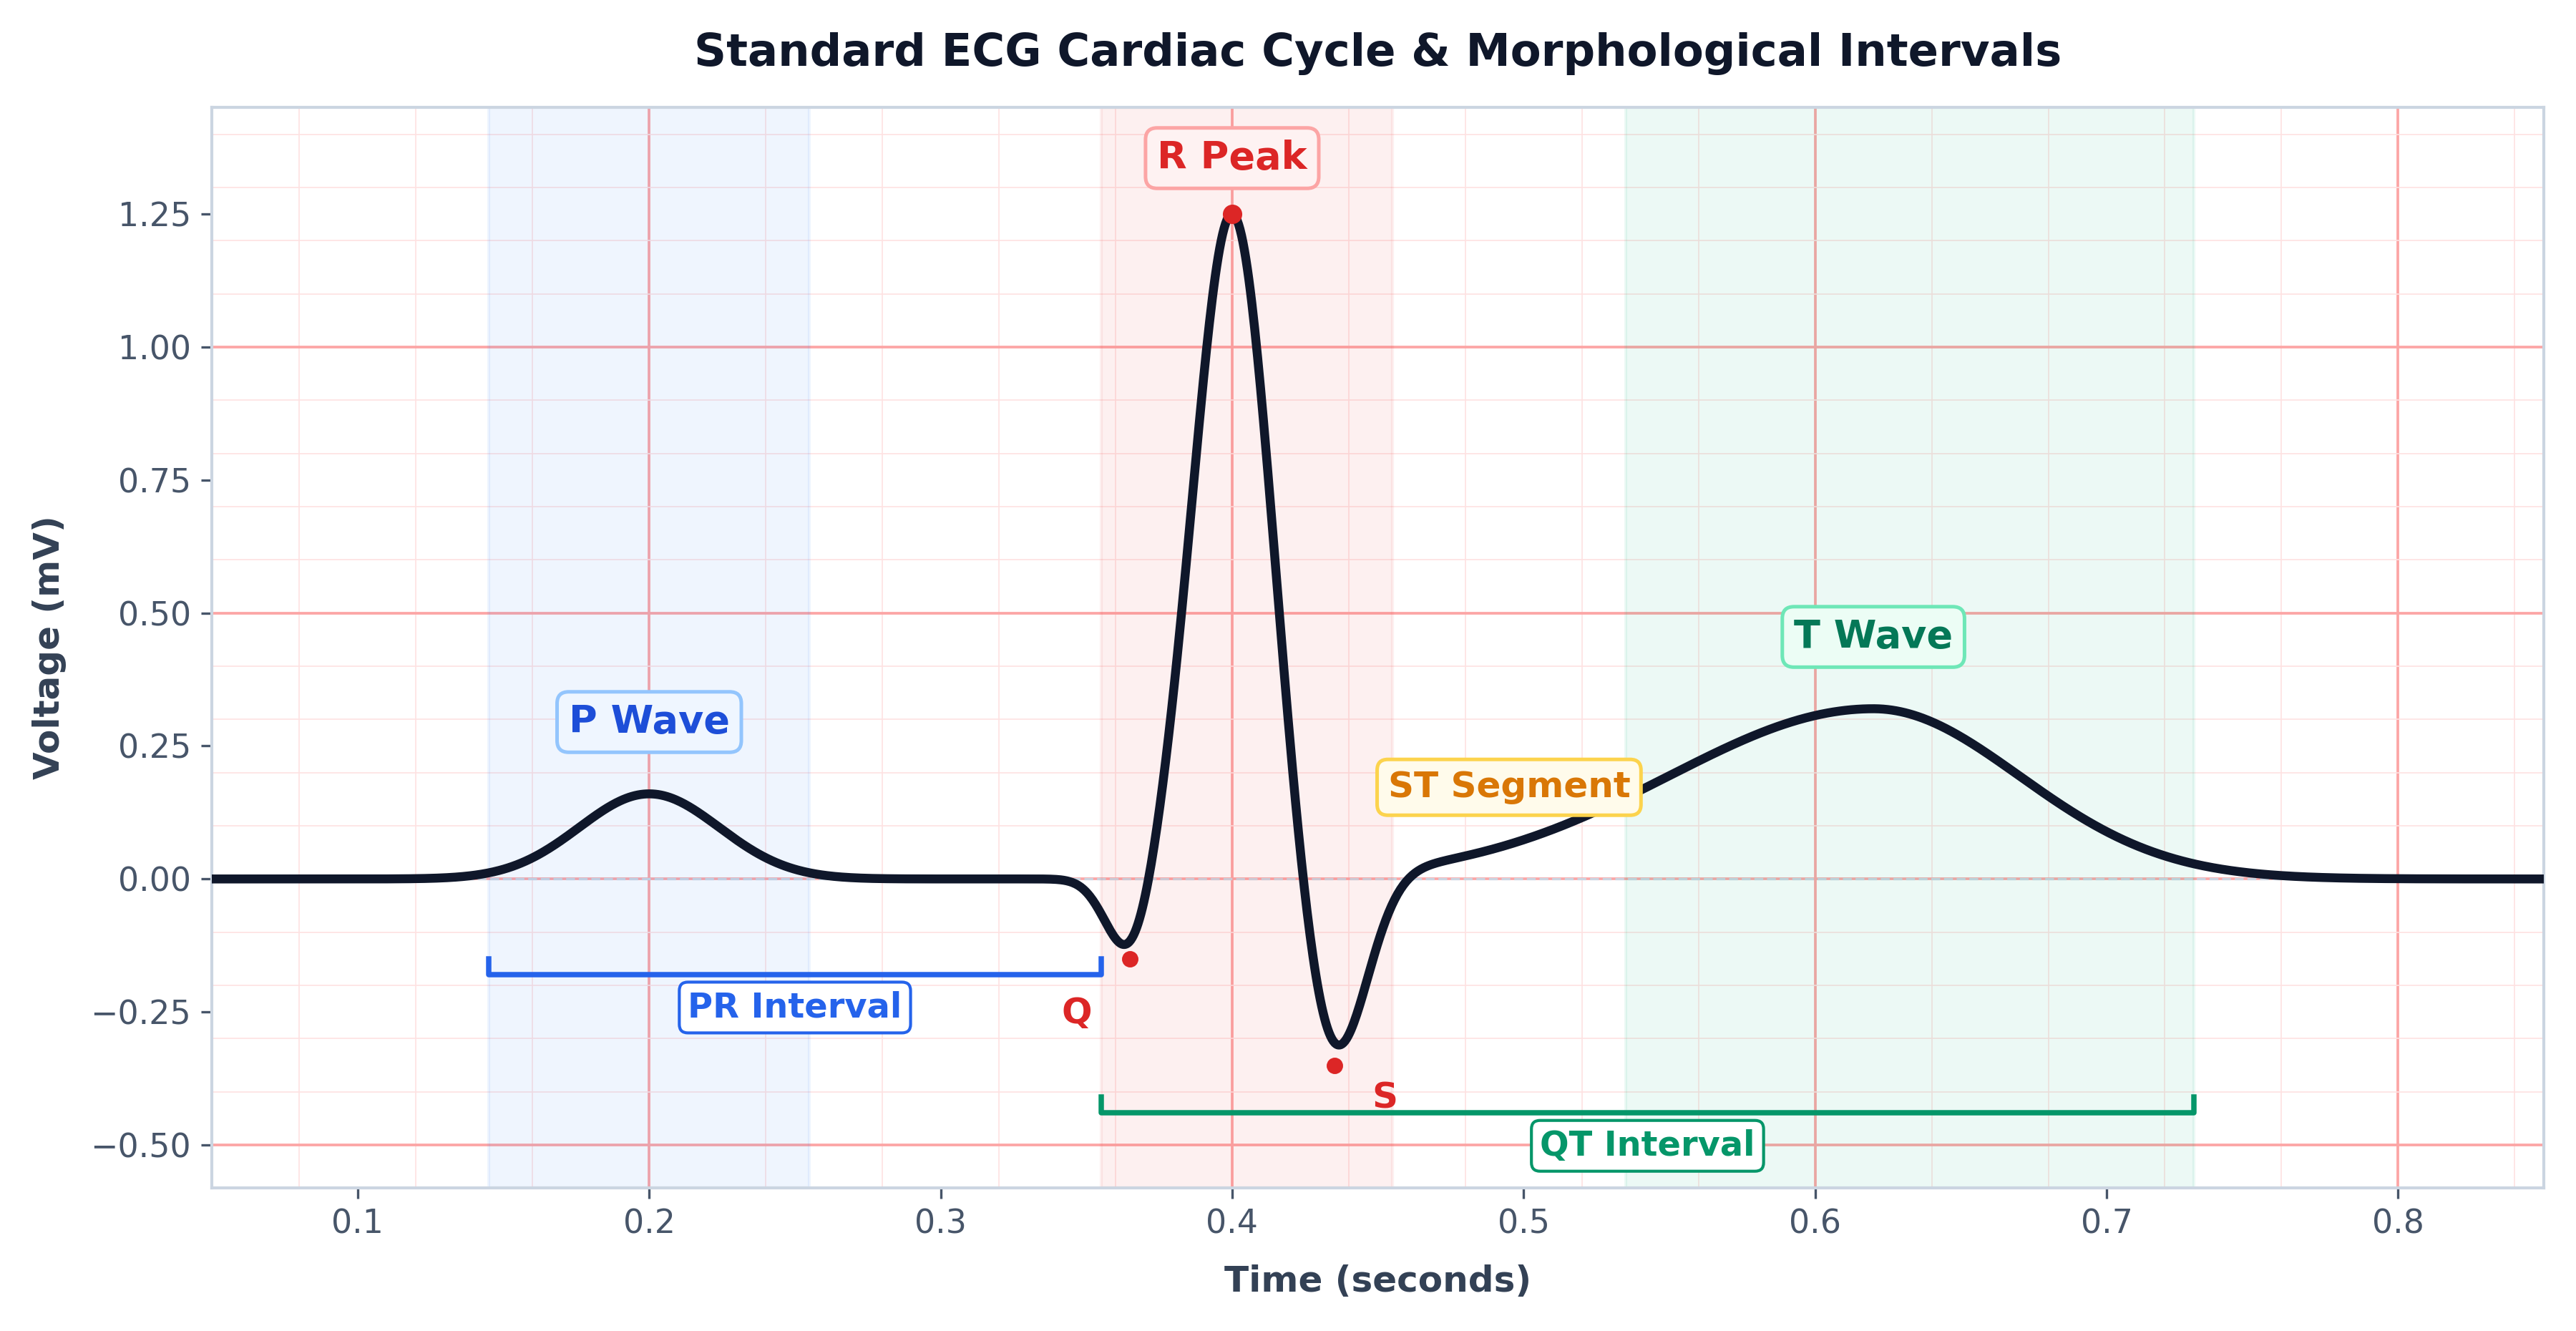
\includegraphics[width=\linewidth,keepaspectratio]{figures/ecg_delineation_components.png}
      \vskip 5pt
      \begin{tcolorbox}[cardstyle,colframe=BorderCol,top=2mm,bottom=2mm]
        \centering\fontsize{8.5}{11}\selectfont
        \textbf{\color{Navy}Electrophysiological Fiducials}\\
        \color{SlateDark}P wave (atria), QRS (ventricles), and ST--T (repolarization)
      \end{tcolorbox}
    \end{column}
    \begin{column}{0.44\textwidth}
      \begin{tcolorbox}[cardstyle,colframe=Navy,top=3mm,bottom=3mm]
        \centering
        {\fontsize{11.5}{14}\selectfont\textbf{\color{Navy}Clinical 12-Lead ECG}\par}
        \vskip 0.2em
        {\fontsize{9.5}{12}\selectfont\textbf{\color{NavyLight}12 Spatial Views}\par}
        \vskip 0.35em
        {\fontsize{8.5}{11.5}\selectfont\color{SlateDark}
        $\cdot$ Frontal (I--aVF) + Precordial ($V_1$--$V_6$)\\[0.25em]
        $\cdot$ Comprehensive 3D cardiac vector field\par}
      \end{tcolorbox}
      \vskip 7pt
      \begin{tcolorbox}[cardstyle,colframe=AlertRed,top=3mm,bottom=3mm]
        \centering
        {\fontsize{11.5}{14}\selectfont\textbf{\color{AlertRed}Smartwatch ECG}\par}
        \vskip 0.2em
        {\fontsize{9.5}{12}\selectfont\textbf{\color{AlertRed}1 Measured Projection}\par}
        \vskip 0.35em
        {\fontsize{8.5}{11.5}\selectfont\color{SlateDark}
        $\cdot$ Single wrist transverse vector (Lead I)\\[0.25em]
        $\cdot$ Completely blind to vertical \& chest planes\par}
        \vskip 0.4em
        {\fontsize{8.5}{11}\selectfont\bfseries\color{AlertRed}
        Most spatial information is unobserved.\par}
      \end{tcolorbox}
    \end{column}
  \end{columns}
  \note{Standard clinical care relies on a twelve-lead ECG, using ten electrodes to capture twelve spatial projections across frontal and horizontal planes. Consumer smartwatches, by contrast, measure only a single projection—Lead I across the wrists. While great for rhythm screening, most spatial information remains completely unobserved.}
\end{frame}

% =========================================================================
% Slide 3: The Reconstruction Challenge
% =========================================================================
\begin{frame}{The Reconstruction Challenge}
  \slideref{Frank, \textit{Circulation} 1956; Atoui et al., \textit{IEEE TBME} 2010.}
  \vspace{0.2em}
  \begin{tcolorbox}[cardstyle,colframe=Navy,top=3.5mm,bottom=3.5mm]
    \centering
    {\fontsize{15}{18}\selectfont
    \textbf{\color{AlertRed}One Observed Lead}
    \quad $\boldsymbol{\longrightarrow}$ \quad
    \fcolorbox{Navy}{LightBg}{\,\textbf{\color{Navy}?}\,\rule[-3pt]{0pt}{16pt}}
    \quad $\boldsymbol{\longrightarrow}$ \quad
    \textbf{\color{SuccessGreen}12-Lead ECG}
    \par}
  \end{tcolorbox}

  \vskip 6pt
  \begin{columns}[T]
    \begin{column}{0.48\textwidth}
      \begin{tcolorbox}[cardstyle,colframe=NavyLight,top=4.5mm,bottom=4.5mm]
        \centering
        {\fontsize{13}{16}\selectfont\textbf{\color{NavyLight}Spatial Ambiguity}\par}
        \vskip 0.5em
        {\fontsize{10}{13.5}\selectfont\color{SlateDark}
        Different cardiac electrical states can produce similar single-lead measurements.\par}
      \end{tcolorbox}
    \end{column}
    \begin{column}{0.48\textwidth}
      \begin{tcolorbox}[cardstyle,colframe=SuccessGreen,top=4.5mm,bottom=4.5mm]
        \centering
        {\fontsize{13}{16}\selectfont\textbf{\color{SuccessGreen}Generative Inference}\par}
        \vskip 0.5em
        {\fontsize{10}{13.5}\selectfont\color{SlateDark}
        The model therefore has to infer plausible missing morphology without simply smoothing it away.\par}
      \end{tcolorbox}
    \end{column}
  \end{columns}
  \note{This creates a fundamental reconstruction challenge: because multiple distinct cardiac electrical states project onto very similar single-lead signals, the problem is underdetermined. Rather than performing simple pointwise regression that averages away critical spikes, the model must infer plausible missing morphology while preserving sharp physiological features.}
\end{frame}

% =========================================================================
% Slide 4: ECG-AIM Model Architecture
% =========================================================================
\begin{frame}{ECG-AIM Model Architecture}
  \slideref{van den Oord et al., VQ-VAE, \textit{NeurIPS} 2017; Ho et al., Axial Attention, \textit{ECCV} 2020.}
  \vspace{-0.7em}
  \centering
  
\includegraphics[width=\linewidth,height=0.82\textheight,keepaspectratio]{figures/conv15e_a0_wave_architecture.png}
  \note{To address this, we developed ECG-AIM. ECG-AIM combines the raw temporal signal with a multiscale wavelet representation, maps these features into a compact latent representation, and jointly reconstructs the missing leads.}
\end{frame}

% =========================================================================
% Slide 5: Experimental Setup
% =========================================================================
\begin{frame}{Experimental Setup}
  \slideref{Wagner et al., PTB-XL, \textit{Sci Data} 2020; Gow et al., MIMIC-IV-ECG, \textit{PhysioNet} 2023.}
  \vspace{-0.2em}
  \begin{columns}[T]
    \begin{column}{0.48\textwidth}
      \begin{tcolorbox}[cardstyle,colframe=Navy,top=3mm,bottom=3mm]
        \centering
        {\fontsize{14}{17}\selectfont\textbf{\color{Navy}$\sim$175k ECGs}\par}
        \vskip 0.25em
        {\fontsize{9.5}{12.5}\selectfont\color{SlateDark}
        Trained and benchmarked across diverse cohorts from \textbf{PTB-XL} and \textbf{MIMIC-IV-ECG}\par}
      \end{tcolorbox}
      \vskip 5pt
      \begin{tcolorbox}[cardstyle,colframe=CyanAccent,top=3mm,bottom=3mm]
        \centering
        {\fontsize{14}{17}\selectfont\textbf{\color{CyanAccent}1 to 3 Observed Leads}\par}
        \vskip 0.25em
        {\fontsize{9.5}{12.5}\selectfont\color{SlateDark}
        Evaluated from single wearable Lead I up to 3 complementary leads (I, II, $V_2$)\par}
      \end{tcolorbox}
    \end{column}
    \begin{column}{0.48\textwidth}
      \begin{tcolorbox}[cardstyle,colframe=NavyLight,top=3mm,bottom=3mm]
        \centering
        {\fontsize{14}{17}\selectfont\textbf{\color{NavyLight}Competitive Baselines}\par}
        \vskip 0.25em
        {\fontsize{9.5}{12.5}\selectfont\color{SlateDark}
        Direct head-to-head comparison against continuous \textbf{1D U-Net} and \textbf{MultiScale-VAE}\par}
      \end{tcolorbox}
      \vskip 5pt
      \begin{tcolorbox}[cardstyle,colframe=SuccessGreen,top=3mm,bottom=3mm]
        \centering
        {\fontsize{14}{17}\selectfont\textbf{\color{SuccessGreen}Comprehensive Evaluation}\par}
        \vskip 0.25em
        {\fontsize{9.5}{12.5}\selectfont\color{SlateDark}
        Evaluated on \textbf{waveform correlation}, \textbf{QRS timing}, and \textbf{downstream clinical preservation}\par}
      \end{tcolorbox}
    \end{column}
  \end{columns}
  \note{We evaluated our framework across 175,000 hospital ECGs from PTB-XL and MIMIC-IV. We tested configurations ranging from one to three observed leads, compared directly against standard continuous 1D U-Net and MultiScale-VAE baselines, and evaluated both raw waveform fidelity and downstream clinical preservation.}
\end{frame}

% =========================================================================
% Slide 6: Spatial Information Determines Reconstruction Quality
% =========================================================================
\begin{frame}{Spatial Information Determines Reconstruction Quality}
  \slideref{Frank, \textit{Circulation} 1956; Atoui et al., \textit{IEEE TBME} 2010.}
  \vspace{-0.6em}
  \begin{columns}[T]
    \begin{column}{0.49\textwidth}
      \begin{tcolorbox}[cardstyle,colframe=SuccessGreen,top=1.5mm,bottom=1.5mm]
        \centering
        {\fontsize{11}{14}\selectfont\textbf{\color{SuccessGreen}3 Leads Acquired (I, II, $V_2$): $r > 0.98$}\par}
        \vskip 1pt
        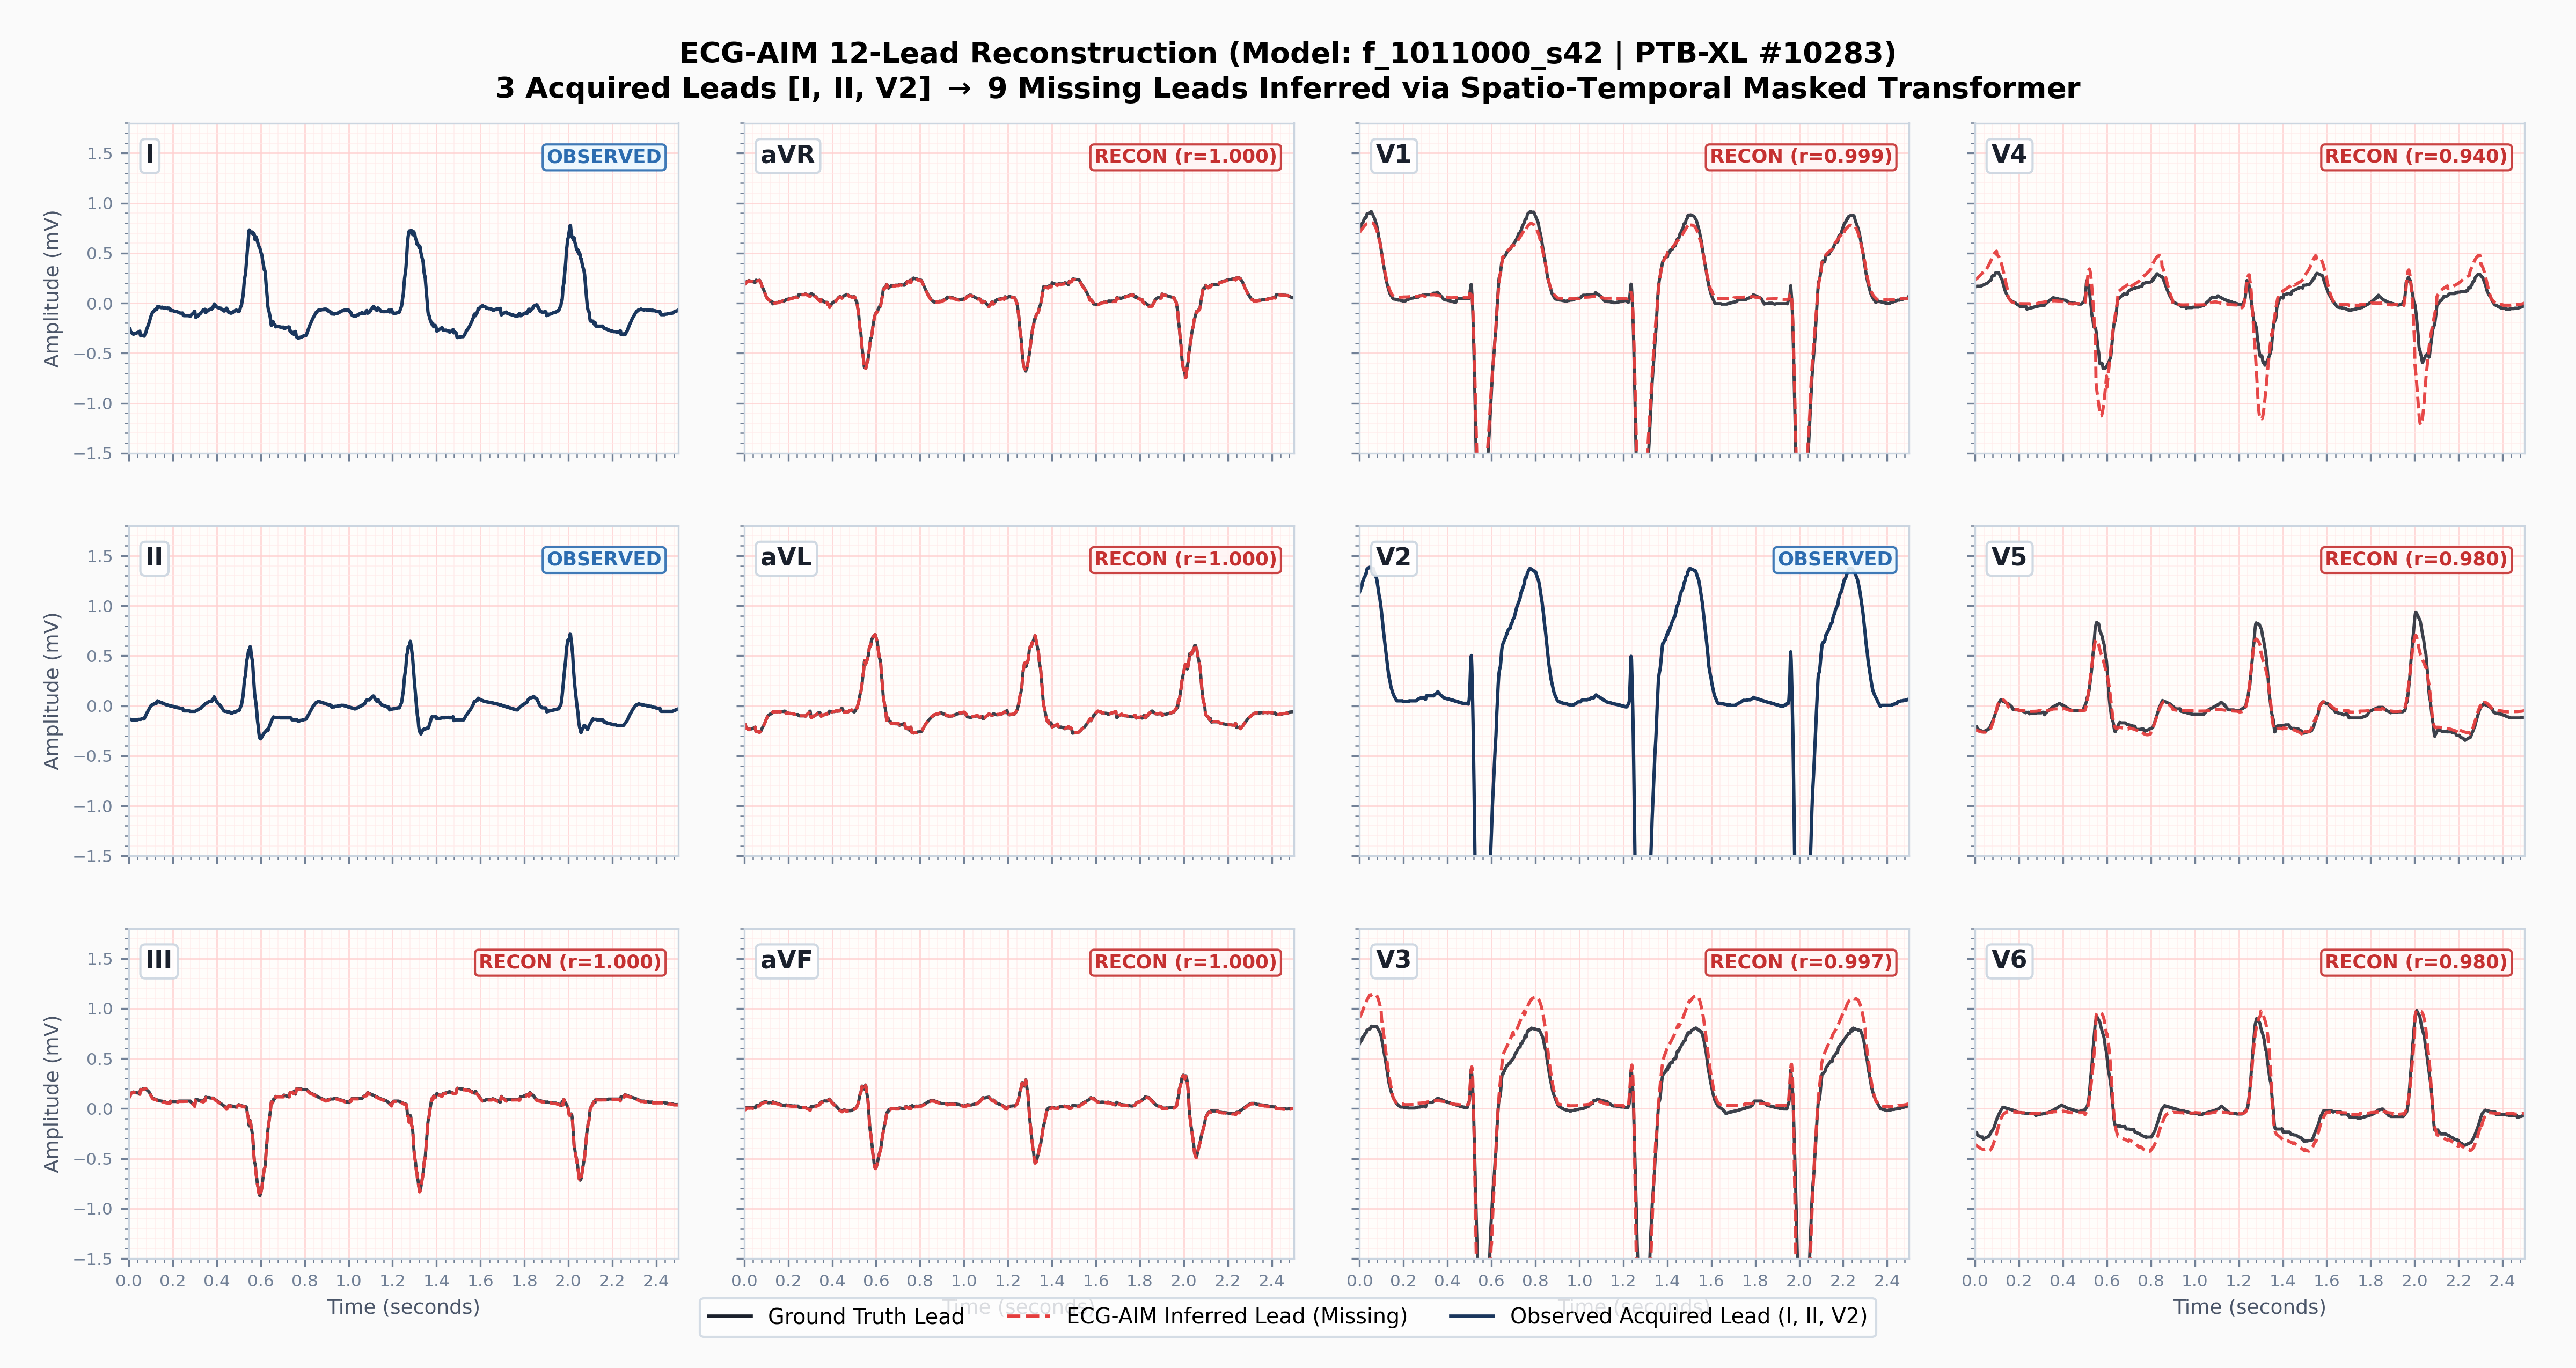
\includegraphics[width=\linewidth,height=0.50\textheight,keepaspectratio]{figures/best_ecg_aim_12lead_reconstruction.png}
      \end{tcolorbox}
    \end{column}
    \begin{column}{0.49\textwidth}
      \begin{tcolorbox}[cardstyle,colframe=NavyLight,top=1.5mm,bottom=1.5mm]
        \centering
        {\fontsize{11}{14}\selectfont\textbf{\color{NavyLight}1 Lead Acquired (Smartwatch Lead I): $r = 0.776$}\par}
        \vskip 1pt
        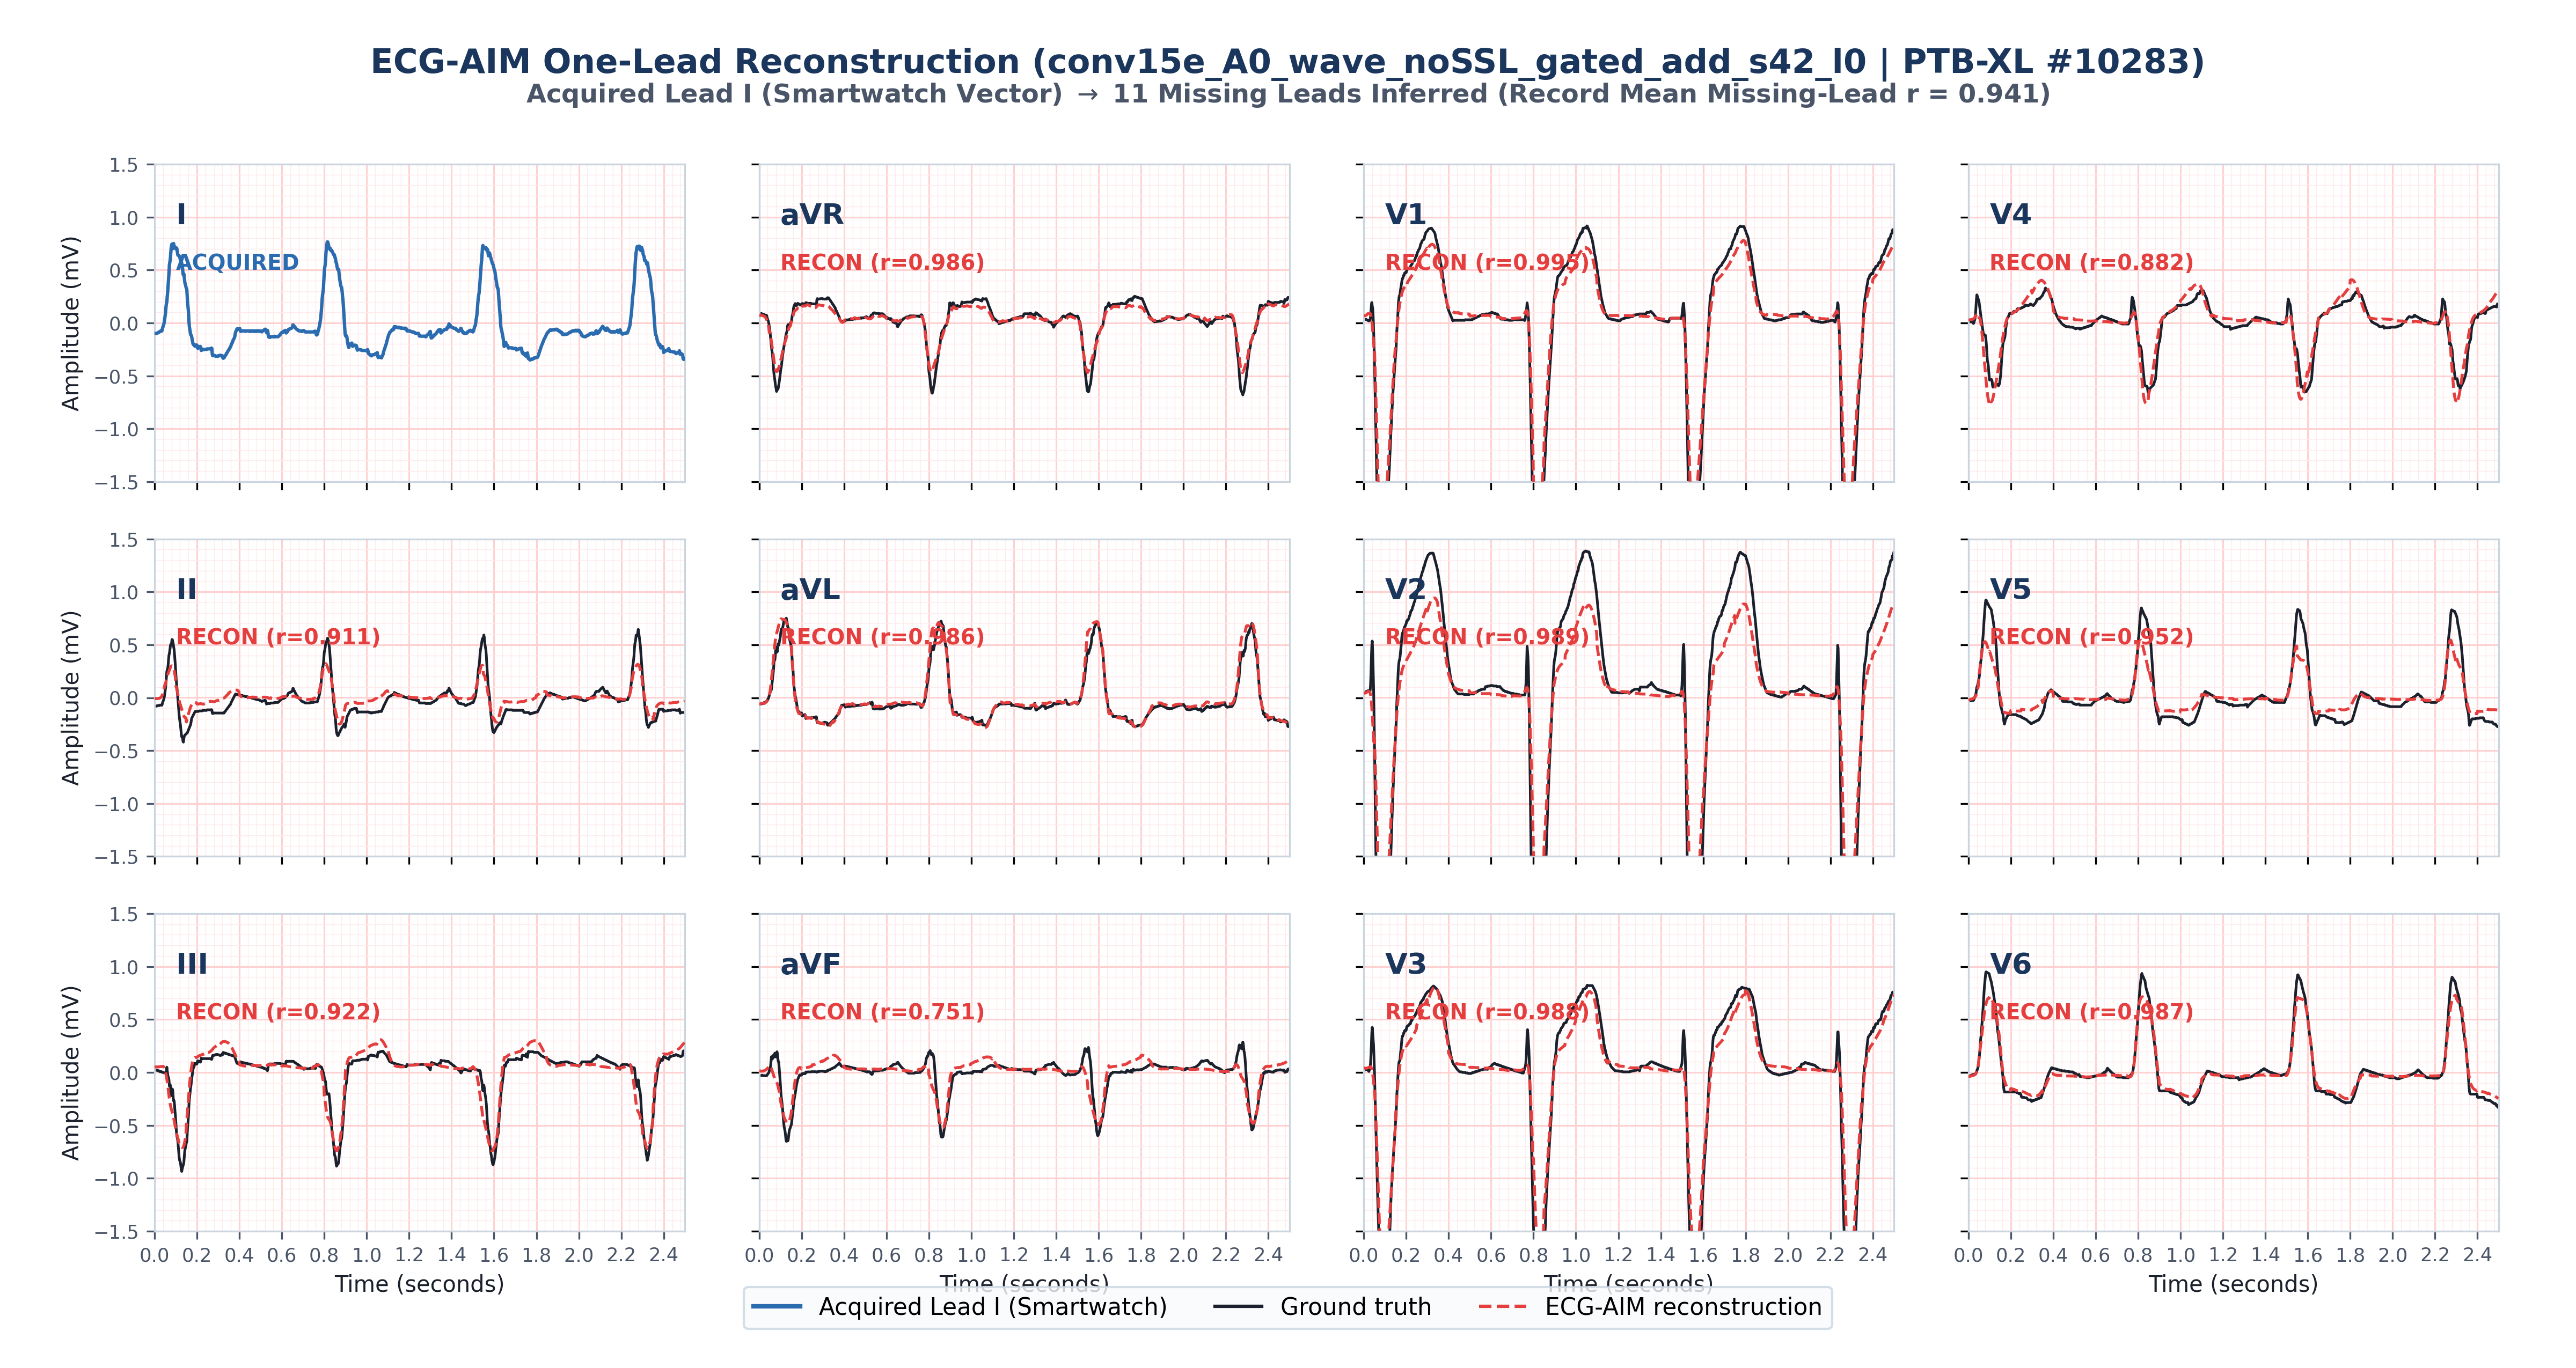
\includegraphics[width=\linewidth,height=0.50\textheight,keepaspectratio]{figures/best_ecg_aim_lead1_reconstruction.png}
      \end{tcolorbox}
    \end{column}
  \end{columns}

  \vskip 3pt
  \begin{tcolorbox}[cardstyle,colframe=SuccessGreen,top=1.8mm,bottom=1.8mm]
    \centering\fontsize{9}{11.5}\selectfont
    \textbf{\color{SuccessGreen}Adding complementary spatial measurements sharply improves reconstruction.} \enspace$\cdot$\enspace
    \color{SlateDark}Spatially complementary leads provide substantially more information for reconstruction.
  \end{tcolorbox}
  \note{With three complementary leads, reconstruction approaches the measured signal. With a single wearable-like Lead I, substantial morphology remains recoverable, but performance falls because the missing spatial information cannot be directly observed.}
\end{frame}

% =========================================================================
% Slide 7: Preservation of Clinically Relevant Structure
% =========================================================================
\begin{frame}{Preservation of Clinically Relevant Structure}
  \slideref{Holste et al., EchoNext Structural Prediction, \textit{JACC Adv} 2024; Surawicz et al., \textit{JACC} 2009.}
  \vspace{-0.2em}
  \begin{columns}[T]
    \begin{column}{0.31\textwidth}
      \begin{tcolorbox}[cardstyle,colframe=Navy,top=4.5mm,bottom=4.5mm]
        \centering
        {\fontsize{12}{15}\selectfont\textbf{\color{Navy}Morphology}\par}
        \vskip 0.6em
        {\fontsize{20}{24}\selectfont\textbf{\color{NavyLight}0.776}\par}
        \vskip 0.3em
        {\fontsize{9}{12}\selectfont\color{SlateDark}
        Precordial Lead $r$\\[0.3em]
        (vs. 0.571 U-Net, 0.684 MS-VAE)\par}
      \end{tcolorbox}
    \end{column}
    \begin{column}{0.31\textwidth}
      \begin{tcolorbox}[cardstyle,colframe=SuccessGreen,top=4.5mm,bottom=4.5mm]
        \centering
        {\fontsize{12}{15}\selectfont\textbf{\color{SuccessGreen}Timing}\par}
        \vskip 0.6em
        {\fontsize{20}{24}\selectfont\textbf{\color{SuccessGreen}8.0 ms}\par}
        \vskip 0.3em
        {\fontsize{9}{12}\selectfont\color{SlateDark}
        QRS Timing Error\\[0.3em]
        (Meets $< 10.0$ ms Clinical Gate)\par}
      \end{tcolorbox}
    \end{column}
    \begin{column}{0.31\textwidth}
      \begin{tcolorbox}[cardstyle,colframe=CyanAccent,top=4.5mm,bottom=4.5mm]
        \centering
        {\fontsize{12}{15}\selectfont\textbf{\color{CyanAccent}Downstream Task}\par}
        \vskip 0.6em
        {\fontsize{20}{24}\selectfont\textbf{\color{CyanAccent}0.775}\par}
        \vskip 0.3em
        {\fontsize{9}{12}\selectfont\color{SlateDark}
        EchoNext Structural AUROC\\[0.3em]
        (Ground Truth = 0.803)\par}
      \end{tcolorbox}
    \end{column}
  \end{columns}

  \vskip 6pt
  \begin{tcolorbox}[cardstyle,colframe=SuccessGreen,top=2.2mm,bottom=2.2mm]
    \centering\fontsize{10}{12.5}\selectfont
    \textbf{\color{SuccessGreen}The reconstruction preserved more than waveform similarity.}
  \end{tcolorbox}
  \note{Crucially, the reconstruction preserved more than waveform similarity. On precordial morphology, ECG-AIM reaches a correlation of 0.776. For clinical timing, it achieves a QRS duration error of 8.0 milliseconds, meeting the clinical gate. And on downstream tasks, EchoNext structural AUROC reaches 0.775, closely tracking the 0.803 ground truth.}
\end{frame}

% =========================================================================
% Slide 8: Conclusions and Translational Next Steps
% =========================================================================
\begin{frame}{Conclusions and Translational Next Steps}
  \vspace{-0.4em}
  \begin{tcolorbox}[cardstyle,colframe=Navy,top=2.2mm,bottom=2.2mm]
    \fontsize{9.5}{12.5}\selectfont
    \textbf{\color{Navy}1. Reconstruction is limited by the spatial information observed.} Single wearable Lead I recovers useful morphology ($r = 0.78$); 3 complementary leads unlock near-lossless recovery ($r > 0.98$).
  \end{tcolorbox}

  \vskip 4pt
  \begin{tcolorbox}[cardstyle,colframe=NavyLight,top=2.2mm,bottom=2.2mm]
    \fontsize{9.5}{12.5}\selectfont
    \textbf{\color{NavyLight}2. ECG-AIM preserves substantial morphology and timing from limited leads.} Reconstructed signals meet clinical timing gates ($8.0\text{ ms}$ QRS error) and retain downstream diagnostic utility ($0.775$ EchoNext AUROC).
  \end{tcolorbox}

  \vskip 4pt
  \begin{tcolorbox}[cardstyle,colframe=SuccessGreen,top=2.2mm,bottom=2.2mm]
    \fontsize{9.5}{12.5}\selectfont
    \textbf{\color{SuccessGreen}3. Prospective paired smartwatch--12-lead validation is the next test.} Translating from retrospective archives to live clinical deployment requires validating across live hardware factors.
  \end{tcolorbox}

  \vskip 6pt
  \centering\fontsize{8}{10}\selectfont\color{SlateMuted}
  \textbf{Sunnybrook paired validation protocol in preparation} \enspace$\cdot$\enspace PI: Dr. Christopher Cheung\\[0.2em]
  \textbf{Mithun Manivannan} \enspace$\cdot$\enspace mithun.manivannan@sri.utoronto.ca \enspace$\cdot$\enspace Abstract \#194
  \note{In conclusion: first, reconstruction is limited by the spatial information observed. Second, ECG-AIM preserves substantial morphology and timing from limited leads. Third, prospective paired smartwatch to twelve-lead validation is our next test. Thank you very much for your attention, and I look forward to your questions.}
\end{frame}

\end{document}
